\documentclass{article}
\usepackage[a4paper, margin=1in]{geometry}
\usepackage{graphicx} 
\usepackage{titling}  
\usepackage{setspace}
\usepackage{indentfirst}
\usepackage{apacite}
\usepackage{newtxtext,newtxmath}
\usepackage{changepage}
\usepackage{csquotes}
\usepackage{enumitem}
\usepackage{hyphenat}
\usepackage{amsmath}
\usepackage{caption}
\usepackage{pdfpages}
\usepackage{graphicx}
\usepackage{caption}
\usepackage{setspace}
\usepackage{float}
\usepackage{booktabs}     % better rules for tables
\usepackage{array}        % advanced column formatting
\usepackage[justification=centering]{caption}
\usepackage{adjustbox} % in preamble
\usepackage{adjustbox}
\usepackage{needspace} % in preamble
\usepackage{booktabs}   % for \toprule etc.

\setlength{\droptitle}{-2cm} % Adjust space before title

\captionsetup{
    font={bf, normalsize}
}

\setlength{\parskip}{1em}
\setlength{\parindent}{0pt}

\begin{document}

\title{Sanctioned but Unshaken: Analyzing the Impacts of the OECD 2000 Sanctions and Resilience of Tax Havens}
\author{Justin Paré, Malachai Ah Yo, Justin Lee, Rohan Kommuri}
\date{\today}

% Use the titling package to place the title
\begin{titlingpage}
    \begin{center}
        \huge \textbf{\thetitle} \\
        \vspace{1em}
    \end{center}


    % Author's name
    \begin{center}
        \Large \theauthor \\[1em]
    \end{center}
    
    % Additional information below the image
    \begin{center}
        \large
        QSS 20 Final Project 
        \vspace{2em}
    \end{center}

% Date
    \begin{center}
        \large June 11, 2025
    \end{center}
\end{titlingpage}


% Table of Contents
% Will automatically update as you add a section/subsection
\renewcommand{\contentsname}{Table of Contents}
\tableofcontents

\newpage
\section*{Abstract}
\addcontentsline{toc}{section}{Abstract}
In this study, we investigated the nature of offshore finances using the dataset published and updated by the International Consortium of Investigative Journalists (ICIJ). Using the information on offshore entities and officers, we analyzed connections between the countries with the most officers and the jurisdictions with the most entities and the mechanisms behind these trends. We also investigated how offshore activity changed before and after sanctions placed by the OECD in 2000. We found evidence that the sanctions were initially successful in lowering offshore activity in the blacklisted regions, but ultimately that activity rebounded as the tax havens fended off the pressure from the OECD. These analyses also highlighted the highly concentrated nature of offshore activity, but also how it is changing and broadening to more jurisdictions. Ultimately, we believe that for tax transparency to increase in these jurisdictions, there needs to be continued research on offshore activity as well as concerted efforts from the world’s largest economies.


\newpage
\section{Introduction}

Corporate tax avoidance through offshore structures and tax havens have emerged as a central concern in contemporary economic and political discourse. Across countries and institutions, growing attention is being paid to the ways multinational corporations and wealthy individuals use shell companies, trusts, and other financial instruments to shift profits and obscure ownership. These practices, though often technically legal, allow for the erosion of domestic tax bases, reduce public revenue, and deepen global inequality. Investigations such as the Panama Papers and Pandora Papers have revealed the scale and sophistication of these networks, showing how secrecy jurisdictions enable corporations to avoid accountability while benefiting from the infrastructure and legal protections of the countries they undercut. Policymakers, economists, and advocacy groups have increasingly called for coordinated reforms to close loopholes, enforce transparency, and promote a tax system that is equitable and resistant to abuse.

Given this growing concern, the International Consortium of Investigative Journalists (ICIJ) has compiled information on more than 810,000 offshore entities that connects companies and individuals to territories/countries from the following investigations that have been made publicly available via leaks:

\begin{itemize}
    \item Pandora Papers (2021)
    \item Paradise Papers (2017-2018)
    \item Bahamas Leaks (2016)
    \item Panama Papers (2016)
    \item Offshore Leaks (2013)
\end{itemize}

In the following paper, we will evaluate the connections and trends between entities and certain geographies, entities and jurisdictions, officer locations and entity locations, and finally, the impact of OECD 2000 sanctions on certain tax haven countries on entity incorporations. It should be noted that named entities/officers in the ICIJ database \textit{does not imply association with criminal activity}, as there do exist legitimate uses for offshore entities.

\section{Related Works}
In June 2000, the Organisation for Economic Cooperation and Development (OECD) published a report titled “Towards Global Tax Cooperation” that marked a pivotal moment in international efforts to address offshore tax avoidance (U.S. Department of State, 2004). In it, the OECD issued a blacklist naming 35 jurisdictions it identified as tax havens—countries or territories with low or zero tax rates, strict bank secrecy laws, and a lack of information exchange agreements (U.S. Department of State, 2004; Sullivan, 2007). These jurisdictions were accused of engaging in “harmful tax competition” by facilitating tax evasion and sheltering income that should be taxed elsewhere (Sullivan, 2007). The OECD threatened to implement “defensive measures” against uncooperative havens by July 2001. These included denying tax deductions and credits for transactions involving tax havens, imposing withholding taxes, and restricting new tax treaties (Sullivan, 2007). While some jurisdictions made early commitments to reform and were spared from the blacklist, others resisted, citing sovereignty and economic survival (Sullivan, 2007). The publication of the list sparked coordinated pushback from tax havens and sympathetic political actors. Ultimately, the campaign lost momentum when the United States reversed its support in 2001 under Treasury Secretary Paul O’Neill, shifting the OECD’s focus/priority from systemic reform to promoting bilateral information exchange agreements—limited in scope and available only upon request (Sullivan, 2007). The automatic information exchange the OECD had been pushing for would have greatly increased tax transparency (Sullivan, 2007). However, set deadlines for reform passed with no consequences for the tax havens, and the OECD ultimately weakened their demands, instead pushing for tax information exchange upon request (Sullivan, 2007). This policy required a formal request with a named taxpayer in order to gain access to information, preserving much of the secrecy that made the tax havens so popular (Sullivan, 2007). The tax havens had won (Sullivan, 2007). However, our study still aimed to see if there were any effects from the OECD 2000 regulations on offshore entity incorporations and inactivations, and if those effects were long lasting.

\section{Data}
This study utilizes the International Consortium of Investigative Journalists (ICIJ) offshore leaks dataset, which is organized as a collection of six interrelated tables. 

For this study, we utilized the ICIJ offshore leaks data in its raw form, which is organized as a collection of six interrelated datasets. Each dataset corresponds to a specific node type or to the set of connections among nodes. Importantly, every record across all six tables is identified by a globally unique node ID, allowing for precise linkage and integration.

Figure 1 illustrates the core relationships between node types. Yellow intermediary nodes are connected to red entity nodes, indicating that a given service provider (e.g., a law firm or trust company) has established or manages the corresponding offshore entity. Green officer nodes link to those same entity nodes as either a shareholder, director, or officer of that entity. Finally, the blue address node is connected to intermediaries, entities, and officers, reflecting the fact that multiple actors often share a common registered office or mailing location.

\begin{figure}[H]
  \centering
    \caption{Database Schema}
  \label{fig:fig1}
  \makebox[0pt][l]{\hspace{-8cm}%
    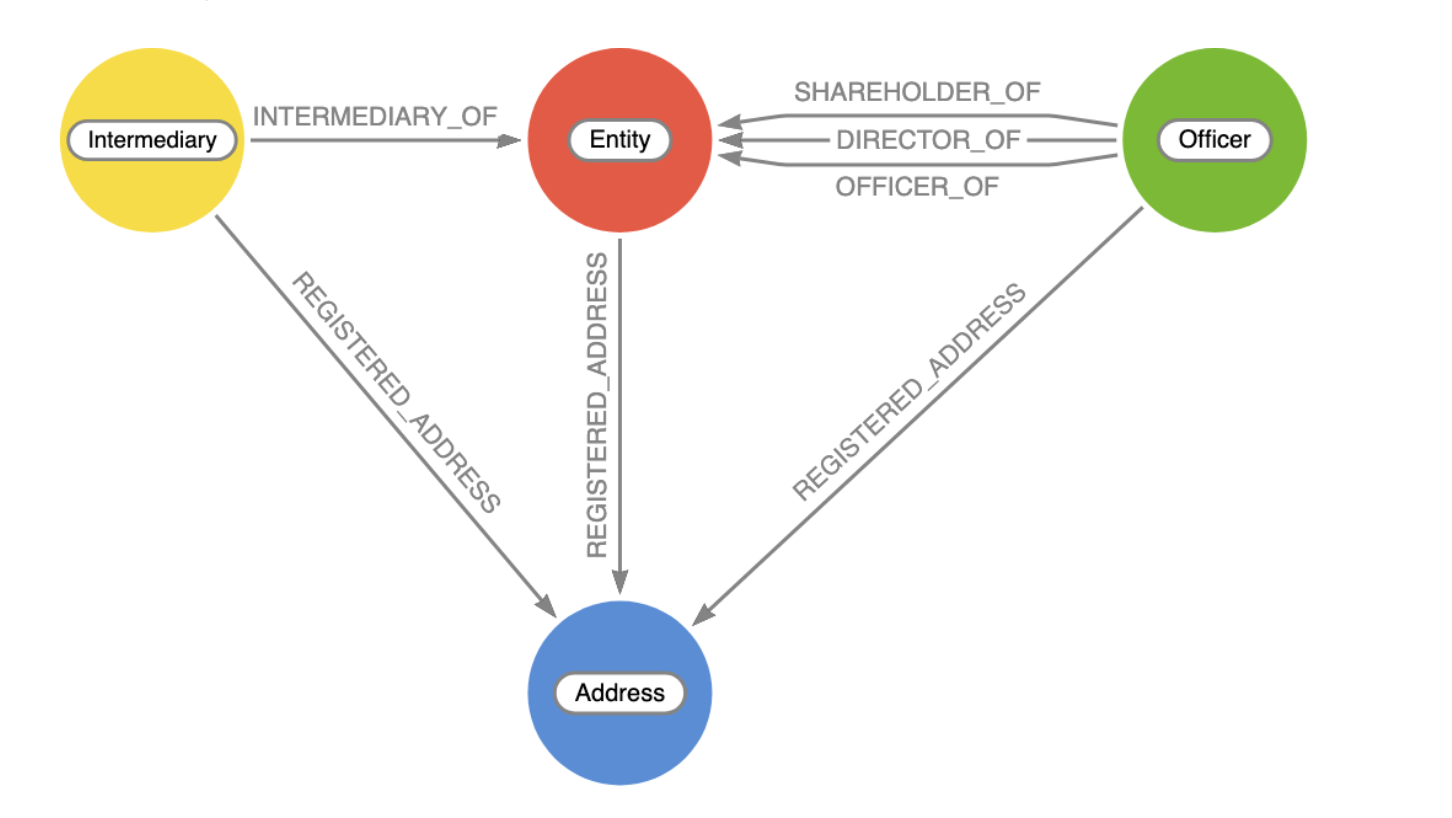
\includegraphics[height=0.4\textheight,keepaspectratio]{figure 1.png}%
  }
\end{figure}


\input{table1.tex}
\newpage

The \textbf{nodes-entities} dataset provides a comprehensive listing of each offshore vehicle, whether a company, trust, foundation, or comparable corporate structure, as a separate row. In its raw form, each record carries a unique node ID alongside key attributes such as the entity’s name, incorporation jurisdiction, registration date, and current status. Because these fields are recorded exactly as in the original export, downstream users can merge entity records unambiguously with related officer, intermediary, and address data.

Similarly, \textbf{nodes-officers} enumerates every individual associated with one or more entities, directors, shareholders, beneficiaries, and nominee directors, preserving raw fields such as name, date of birth (when available), nationality, and specific officer role. Each officer also has a unique node ID, enabling researchers to trace precisely which individual serves which entity. In parallel, nodes-intermediaries.csv captures every service-provider organization involved in establishing or managing offshore entities, law firms, trust companies, nominee director services, and other corporate service outfits. Here, each intermediary node retains raw attributes like provider name, jurisdiction, and service type, with the node ID facilitating direct linkage to the entities they helped create or continue to oversee.

The \textbf{nodes-addresses} dataset remains unaltered from the original export, cataloging all physical and mailing locations, registered offices, forwarding-service addresses, and so on, tied to entities, officers, and intermediaries. Because each address node includes street lines, city, region or state, postal code, and country exactly as provided by the leak, analysts can use these records to detect geographic clustering or shared domiciles among multiple nodes. 

Meanwhile, \textbf{nodes-others} functions as a catch-all repository for any remaining node types that do not fit neatly into the categories of “entity,” “officer,” “intermediary,” or “address.” Examples in this table include jurisdiction-registry nodes (such as “BVI Registry” or “Panama Public Registry”) and standalone document nodes that the import pipeline treated as discrete items. Each “other” node retains its original ID and type label, preserving the raw context in which it appeared.

Finally, the \textbf{relationships} file serves as the unprocessed edge list that binds all node tables into a cohesive graph. Each row specifies a “start” node ID and an “end” node ID, together with a raw relationship type, such as officer\_of, registered\_address\_for, or intermediary\_for, and includes “start\_date” and “end\_date” fields indicating the active period of that connection. By merging node IDs from the other five nodes tables with the relationships file, it is possible to reconstruct the full, unaltered network of offshore linkages: identifying who is connected to whom, in what capacity, and over which time span.

\section{Methods}
\subsection{Data Merging}
To merge the datasets, we first loaded each of the six node files (nodes-addresses, nodes-entities, nodes-intermediaries, nodes-officers, and nodes-others) directly into memory. For every file, we immediately added a new column called node\_type, assigning values such as address, entity, intermediary, officer, or other to clearly mark each record’s origin. This step ensured that when we later concatenated all five node-specific data frames, we would still know which original table each row came from. After tagging, we concatenated these data frames into a single nodes table. By unifying them, we created a master catalog of every node in the network, regardless of type, while still preserving the ability to filter or group by node\_type if needed.

Next, we loaded the relationships file, which contains every pair of connected node IDs under the columns node id start and node id end, representing directed edges in the offshore network. To enrich the relationships table with metadata, we performed two sequential left joins against our combined nodes table. In the first join, we matched node id start from relationships to node id in the nodes table and appended suffixes like \_start to each merged column (for example, name\_start, jurisdiction\_start, and node\_type\_start). In the second join, we matched node\_id\_end to the same nodes table and suffixed those columns with \_end (for example, name\_end, jurisdiction\_end, and node\_type\_end). By adding these suffixes, we kept all merged fields clearly organized in each resulting row. The outcome was a fully enriched edge list in which every single relationship record carried complete metadata for both the start and end nodes, enabling us to trace, in one cohesive table, exactly which entity, officer, intermediary, address, or other node appeared at each end of every connection.

\subsection{Data Cleaning}
To clean the merged dataset, we first removed any duplicate rows that had arisen during the merging process. By comparing every column in each record, we dropped exact matches so that each relationship between nodes appeared only once. This deduplication step was crucial to prevent overcounting edges and to ensure that our analysis reflected unique connections rather than repeated entries.

Next, we standardized all textual fields to eliminate subtle inconsistencies. We collapsed consecutive spaces into a single space, trimmed leading and trailing whitespace, and stripped out stray punctuation using regular expressions. For instance, we ran each object-type column through a pattern that replaced multiple whitespace characters with one space and then applied a trim operation. These cleaning steps ensured that values such as “ Offshore Entity ”, “offshore-entity”, and “Offshore Entity” were all normalized to the same format. As a result, our dataset no longer contained artificial distinctions caused by extra spaces or punctuation, allowing us to group and compare names, jurisdictions, and other text fields reliably.

Additionally, for the investigations into the OECD 2000 sanctions, we only needed all the unique entities along with jurisdiction and date information, so we opted to use the nodes-entities dataset directly. While node-id was able to be used directly for tracking and counting unique entities, the jurisdiction\_description field needed to be cleaned. Comparing a list of the blacklisted jurisdictions with all the unique jurisdiction-description values allowed us to determine how we needed to clean the column’s data. The function we created to clean the data made every description lowercase, stripped white space and newline characters, and replaced “\&” with “and”. Additionally, there were other features to be cleaned specific to this dataset. For one, “british anguilla” was replaced with just “anguilla.” “St.” (with period) and “st” (without period) were also both replaced with “saint.” Additionally, “u.s.” was replaced with “us”, “cookislands” was replaced with “cook islands”, and “nevis” was replaced with “saint kitts and nevis.” This way, we could accurately count the entities in each jurisdiction and avoid splitting a jurisdiction’s entity count into two groups with slightly different spellings of the jurisdiction.

Other columns in the node-entities dataset also needed to be cleaned. For instance, we created a time-series graph looking at the levels of newly incorporated entities as well as inactivated entities for the blacklisted jurisdictions around the year 2000. To do this, we filtered for entities that had both an incorporation start date, as well as an inactivation/struck off date or an “active status.” To accomplish this, we created date objects from the incorporation\_date, inactivation\_date, and struck\_off\_date columns. We used the year from incorporation\_date as the incorporation year for the analyses. However, for the end date, we took the minimum of the inactivation\_date and struck\_off\_date as the end date. If values were missing from both columns, we also checked the status column to see if the entity was still active. After looking at all the unique values in the status column and stripping them of whitespace and putting them in lowercase, we considered only those entities labeled as “active” or “open” to be still active. Altogether, only those entities with an incorporation date as well as an inactivation or struck off date or active status were included in the time series graph. However, other analyses that only needed to include the incorporation date were filtered differently, only filtering out entities without an incorporation date.

\subsection{Initial Findings}
When initially looking at the data, we first wanted to isolate every direct link between an offshore entity and its registered address so we can map the top 10 most popular countries for entities to be based out of. 
To do this, we filtered for relationships where node\_type\_start == entity and node\_type\_end == address, then counted the number of unique entities per destination country. Along with this, we also looked at the top 10 most popular jurisdictions in the entities dataset. Looking at the plot we made, we noticed that the BVI, Malta, Barbados, and the Bahamas, seemed to dominate the offshore wealth network.

\subsection{Analyses Plan}
We hoped to distill the Offshore Leaks network into a single two‑level Sankey diagram. Our goal was to map the five most common officer countries (Hong Kong, Switzerland, Jersey, Luxembourg and the United Kingdom) to the five most frequent entity\_jurisdictions (Malta, the British Virgin Islands, Barbados, the Bahamas and Panama). In essence, this graph represents the relationship between the officer’s origin country and the location in which the company that officer belongs to is located. Because the same place can serve simultaneously as an officer domicile and an incorporation venue, this diagram also showed “self‑loops”. An example of this being how Malta’s massive volume of recorded links connect Maltese officers back to Maltese entities.

Along with this, we wanted to compare annual incorporations and closures before and after the OECD’s 2000 blacklist to see if blacklisted havens experienced a breakpoint in activity. By focusing on Malta, the BVI, and the Bahamas, we aimed to uncover the regulatory and commercial factors, nominee requirements, citizenship-by-investment programs, and transparency reforms, that drive both the self-loop behavior and shifts in offshore registration trends.

\section{Results}
\subsection{Review of Initial Findings}

\begin{figure}[H]
  \centering
    \caption{} 
  \label{fig:fig2}
  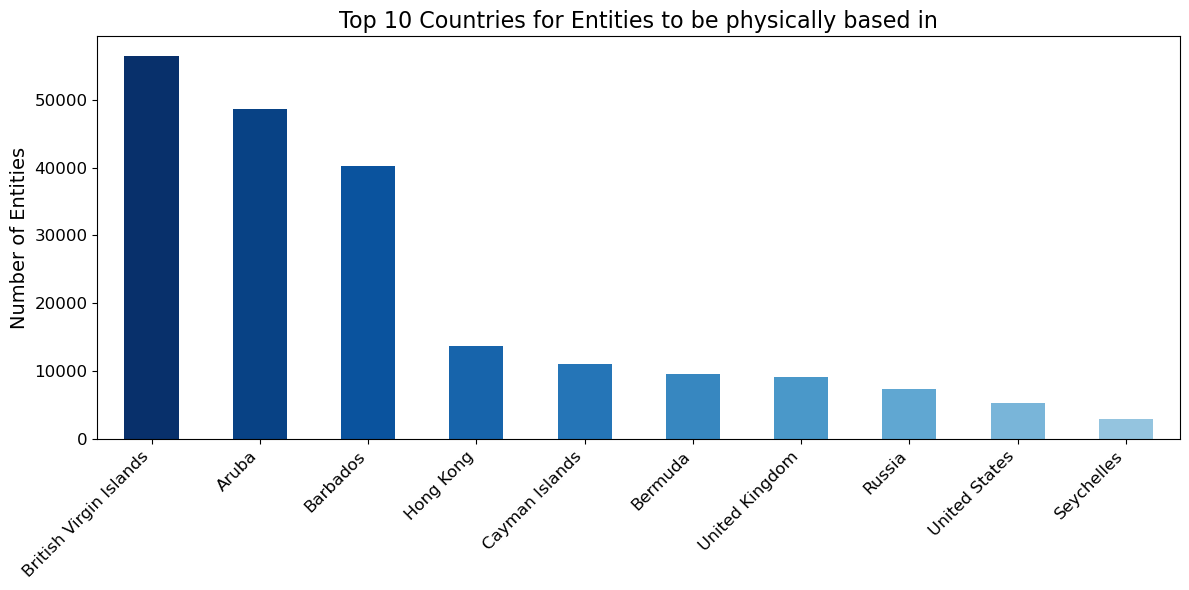
\includegraphics[width=\textwidth]{Figure 2.png}
\end{figure}

As shown in Figure 2, the distribution is heavily skewed: the British Virgin Islands, Aruba, and Barbados alone account for the lion’s share of entity registrations, with a steep drop-off after the third rank. This pattern reflects a classic power-law distribution, where a few jurisdictions dominate the global network of registered offices. The presence of large economies such as the United Kingdom and the United States in the lower decile highlights that offshore structuring extends beyond small island states.

Next, we turned to the legal domiciliation of entities by tallying the incorporation jurisdictions recorded in the raw entity table.

\begin{figure}[H]
  \centering
  \caption{} 
  \label{fig:fig3}
  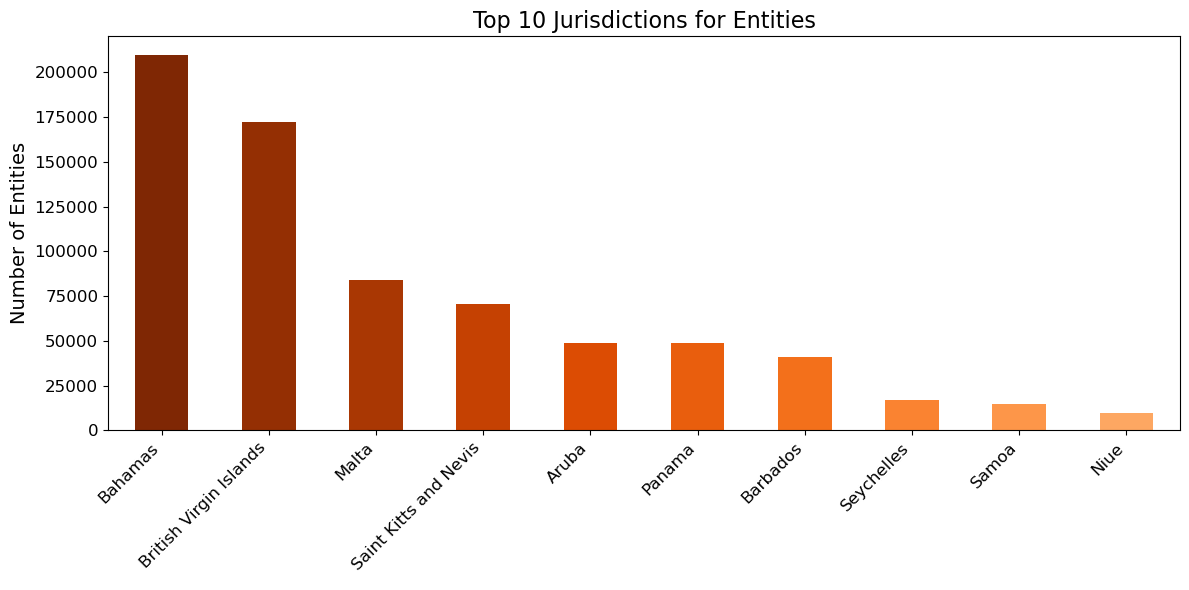
\includegraphics[width=\textwidth]{Figure 3.png}
\end{figure}


The Bahamas and the British Virgin Islands emerge as the predominant legal homes, followed by Malta, Saint Kitts and Nevis, and other small, low-tax jurisdictions. Again, the curve follows a power-law shape: a handful of jurisdictions host the overwhelming majority of corporate vehicles, while dozens of others see only minimal use. This reinforces the notion of a highly concentrated legal framework that underpins offshore finance.

To investigate how offshore activity is distributed across jurisdictions and intermediaries, we examined officer-entity relationships and the locations in which 1) officers are from and 2) entities are registered. Specifically, we mapped each officer’s country of residence to the jurisdiction where the associated entity is incorporated, allowing us to observe cross-border registration patterns and identify which territories attract the most foreign-linked entities. A Sankey diagram was well suited for this analysis because it effectively visualizes the magnitude and direction of flows between officer countries and entity jurisdictions, allowing us to capture both the volume and concentration of connections within the offshore network. Looking at the Sankey graph in Figure 4, and the bar chart in Figure 5, three patterns stand out. First, Malta eclipses the traditional Caribbean havens, drawing a large share of officers and entity jurisdiction connections (mostly self connections). Second, the British Virgin Islands remains a major offshore hub, the red band loops heavily on itself and still attracts sizeable inflows from Switzerland, Hong Kong, and Jersey, yet its absolute volume in our filtered sample is barely half of Malta’s. Third, focusing specifically on the sankey graph in Figure 3, flows are highly concentrated: outside the five highlighted jurisdictions, more than 190 other entity locations identified in nodes‑entities account for less than 30\% of officer links, underscoring just how narrow the practical menu of offshore options has become. These relationships lead us to believe that the officers who are running these companies, although registered as living in countries like Malta, the BVI, Barbados, Bahamas, and Panama, are not actually located there (for example, Malta’s total population is 500,000). 


\begin{figure}[H]
  \centering
    \caption{} 
  \label{fig:fig4}
  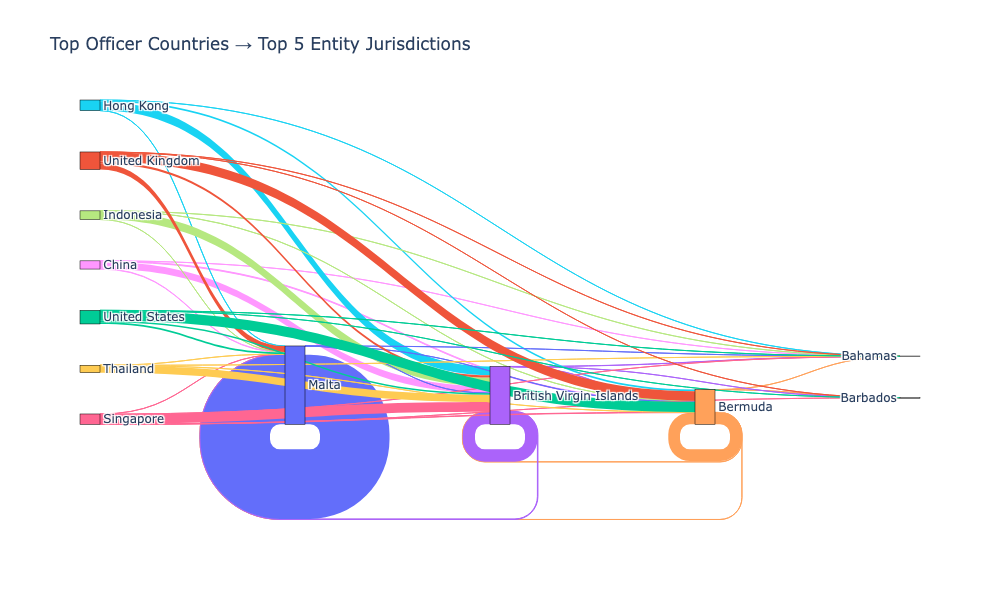
\includegraphics[width=\textwidth]{Figure 4.png}
\end{figure}

\begin{figure}[H]
  \centering
    \caption{} 
  \label{fig:fig5}
  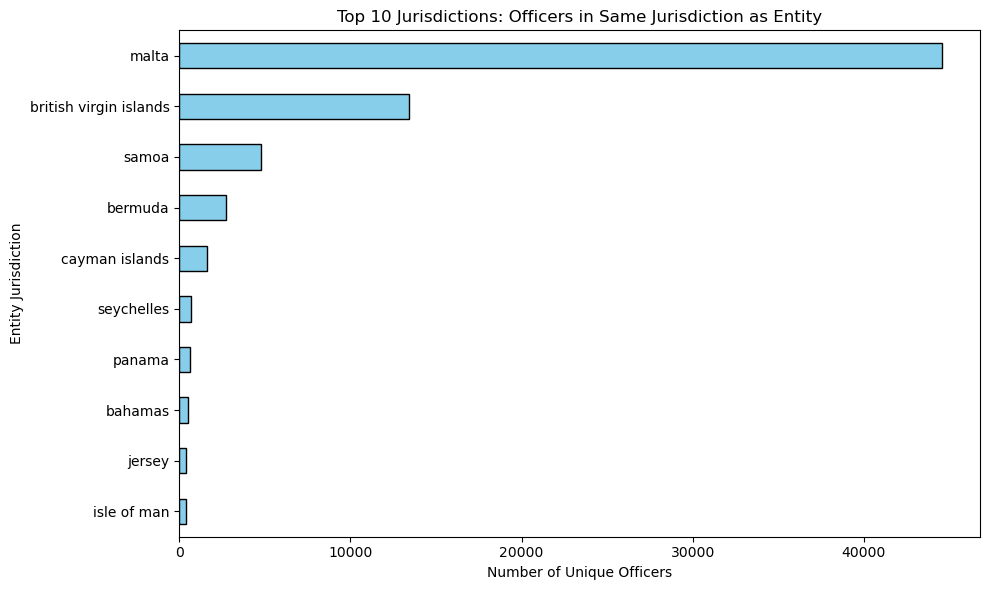
\includegraphics[width=\textwidth]{Figure 5.png}
\end{figure}

\subsection{OECD Findings}

\begin{table}[H]
  \centering
  \caption{} 
  \label{fig:table2}
  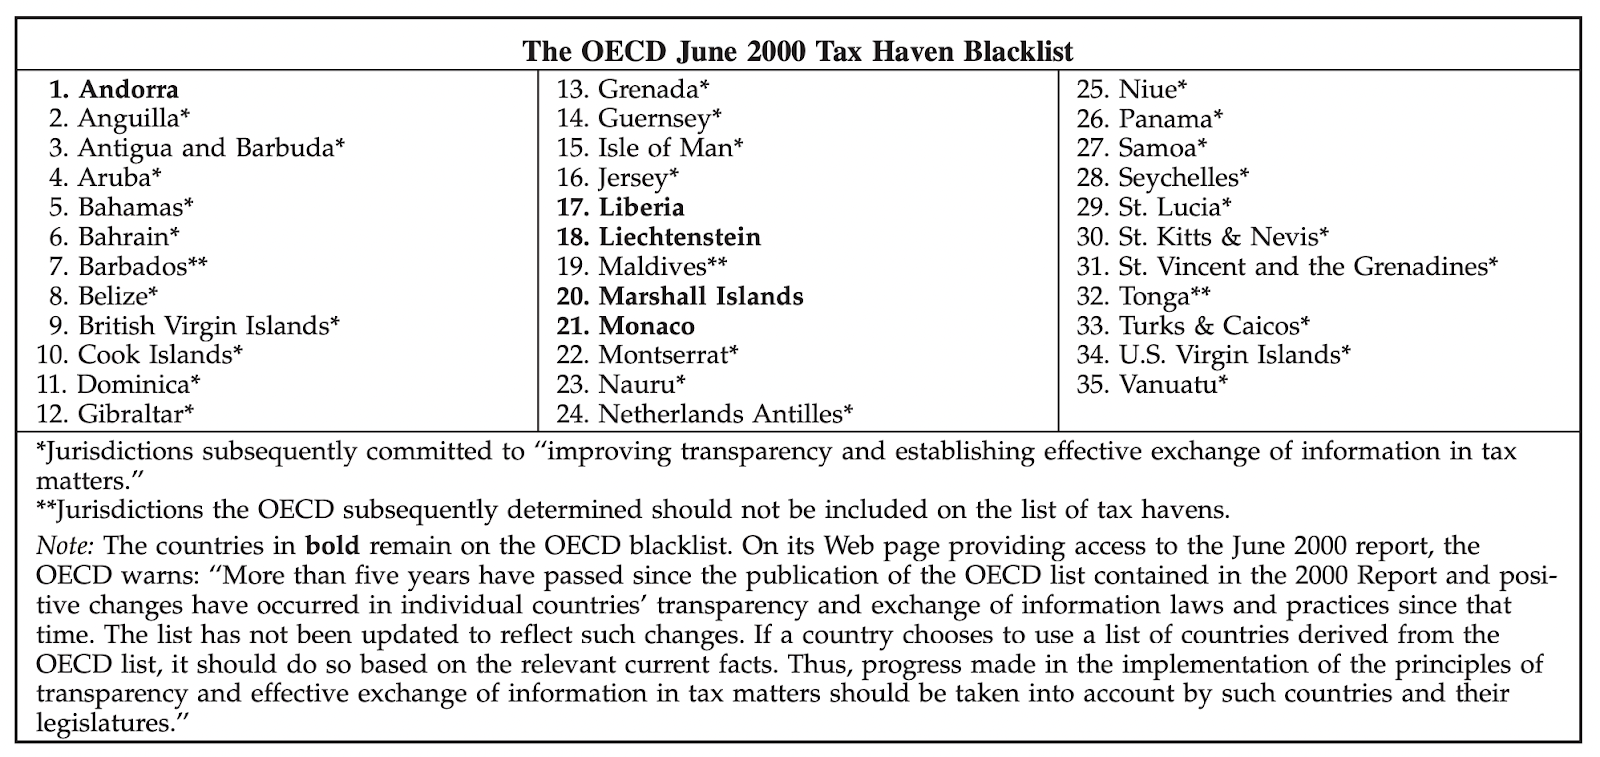
\includegraphics[width=\textwidth]{Table 2.png}
\end{table}

\begin{figure}[H]
  \centering
    \caption{} 
  \label{fig:fig6}
  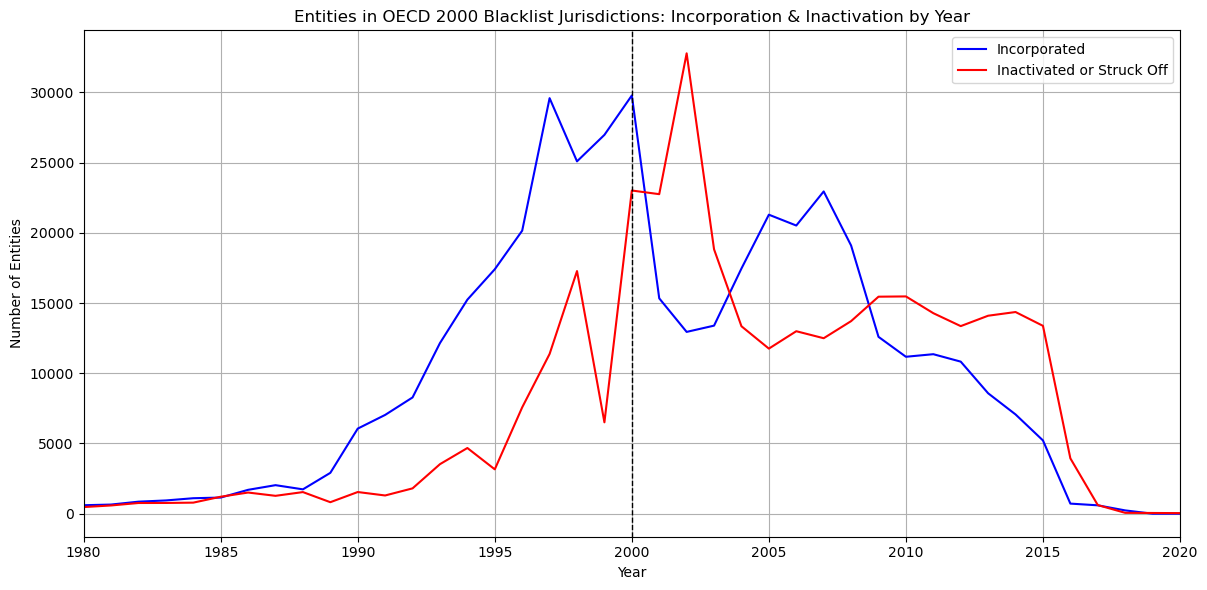
\includegraphics[width=\textwidth]{Figure 6.png}
\end{figure}

To assess the impact of the OECD’s 2000 initiative, we examined trends in the incorporation and inactivation of entities across the 35 jurisdictions named in the blacklist. As shown in Figure 6 above, the number of newly incorporated entities (the blue line) rose steadily throughout the 1990s, peaking in the late 1990s at nearly 30,000 entities per year. Beginning in 2000, the year the OECD published its report, incorporations declined sharply. At the same time, the number of entities that were inactivated or struck off (the red line) increased substantially, reaching a historic peak in 2001.

This reversal of trends suggests a reaction to the OECD’s announcement. However, the lag between the report’s release and the observed changes in activity, particularly the peak in inactivations occurring in 2001, indicates that the effects may not have been immediate. The dissolution of entities likely followed internal reassessments by firms and intermediaries in response to growing regulatory uncertainty, reputational risk, or anticipated policy changes. The spike in inactivations occurring after rather than during 2000 may reflect the time required to wind down offshore structures or for the implications of the blacklist to be fully absorbed by affected actors.

Looking at the sharp increase in inactivations from 2000-2003 as well as the rebound in new incorporations from 2004-2007, we took a closer look at the top jurisdictions involved in these trends, as seen in Figure 7 and 8 below. The first graph highlights the top 10 jurisdictions on the blacklist with the greatest number of inactivated entities from 2000-2003. The second graph displays the top 10 jurisdictions on the blacklist with the greatest number of newly incorporated entities from 2004-2007. Both graphs display the values as proportions of the overall number of inactivations and new incorporations in the respective time periods. As we saw in other analyses, the graphs follow a power law distribution, again highlighting the highly concentrated nature of offshore finances.From 2000-2003, the Bahamas was by far the jurisdiction with the highest number of inactivated entities with over 60\% of the total, which we suspect was due to the OECD 2000 regulations. BVI had the third highest number of inactivated entities, comprising around 15\% of the total number. On the other hand, BVI was the most popular jurisdiction for new incorporations from 2004-2007, comprising around 45\% of the total share. Meanwhile, the Bahamas was only the 4th most popular jurisdiction for new incorporations.


\begin{figure}[H]
  \centering
    \caption{} 
  \label{fig:fig7}
  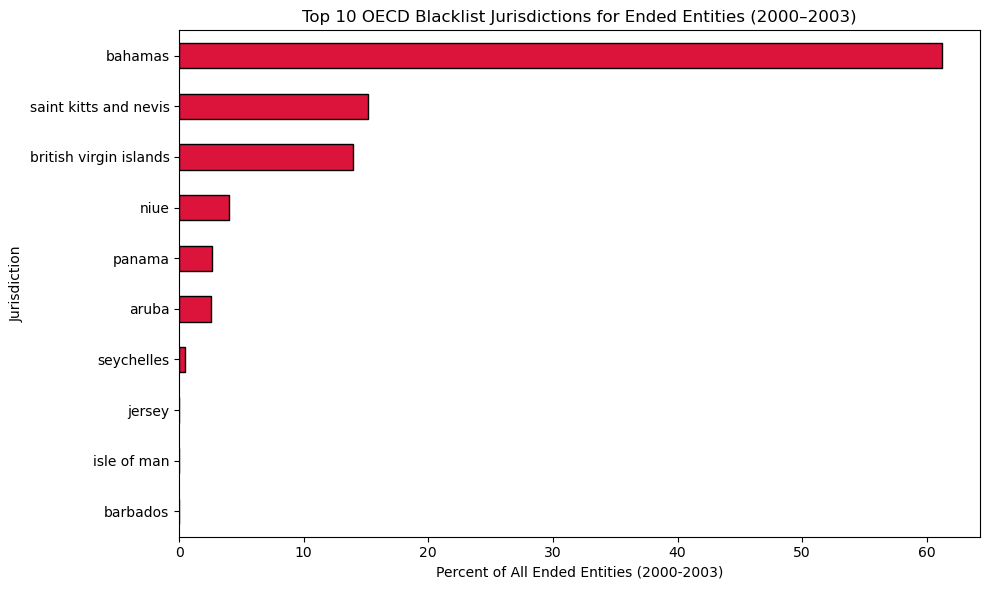
\includegraphics[width=\textwidth]{Figure 7.png}
\end{figure}

\begin{figure}[H]
  \centering
    \caption{} 
  \label{fig:fig8}
  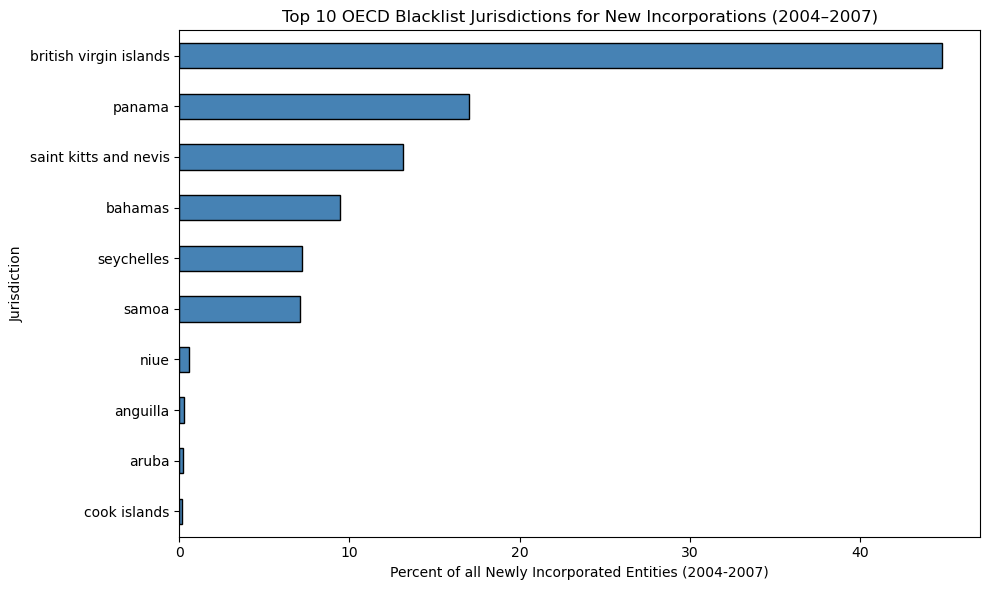
\includegraphics[width=\textwidth]{Figure 8.png}
\end{figure}

To further investigate the dynamic landscape of offshore finances, especially with regard to the OECD blacklist, we constructed two more graphs, one displaying the top 10 jurisdictions for new incorporations prior to 2000, and the other the top 10 jurisdictions for new incorporations after 2007. For this analysis, all jurisdictions were included, not just those on the blacklist. The year 2007 was used because at this point, only four territories (none of which appeared on either top 10) were still on the blacklist, while others were either removed or had made commitments to comply with (albeit weakened) regulations (Sullivan, 2007). It is important to note that since these analyses were not directly related to the findings of the time-series graph here, a different filtering process was used. Instead of filtering for entities with both incorporation and “end” dates, we only filtered for entities with incorporation dates. Interestingly, when conducting the analysis, we first conducted it on the data filtered for entities with both incorporation and end dates. When we switched to a filtering strategy that only required entities to have incorporation dates, Malta appeared in both top tens, where it was on neither with the overly conservative filtering. The incomplete nature of our dataset is important to consider when interpreting our findings.

\begin{figure}[H]
  \centering
    \caption{} 
  \label{fig:fig9}
  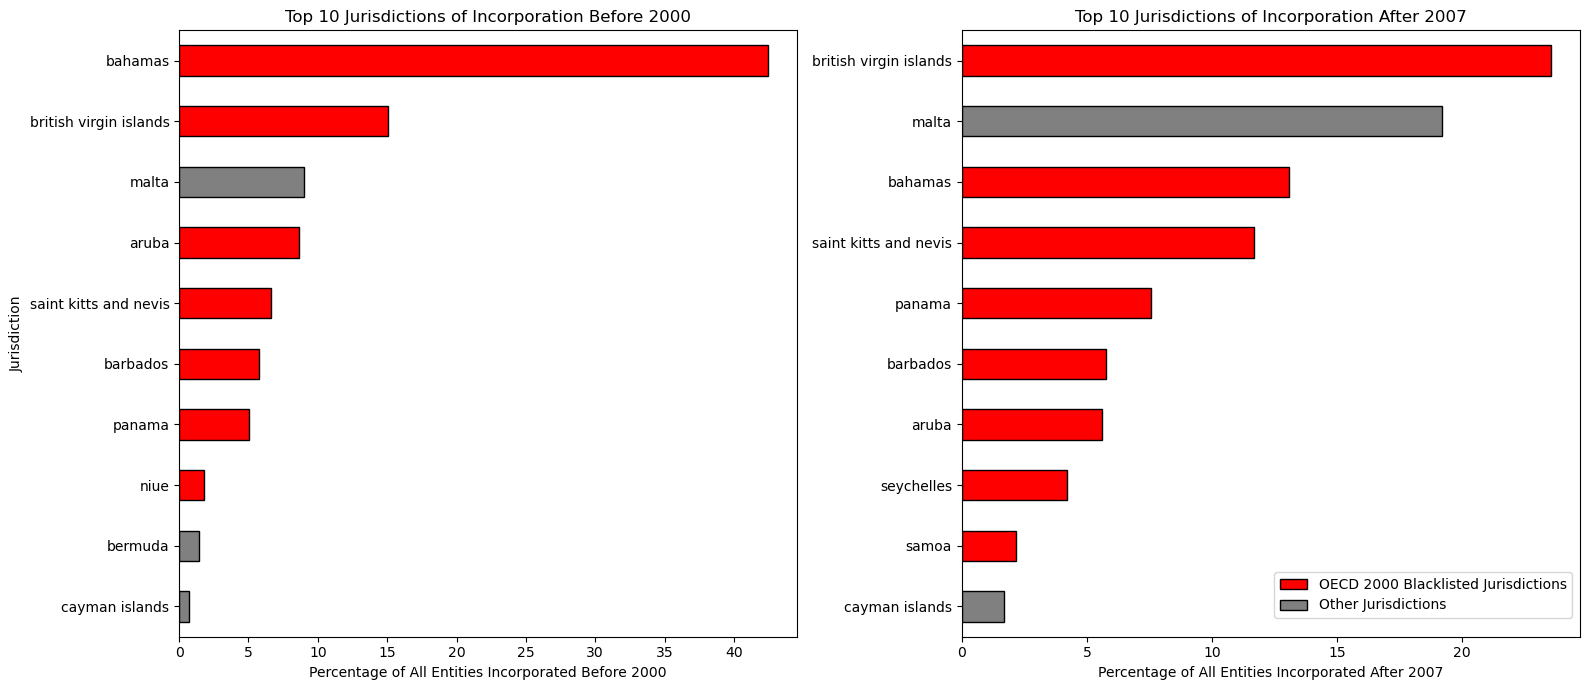
\includegraphics[width=\textwidth]{Figure 9.png}
\end{figure}

Once more, both graphs followed a power law distribution, however, the distribution of new incorporations after 2007 was less concentrated compared to before 2000. The most popular jurisdiction for incorporation before 2000 garnered over 40\% of the total share. Meanwhile, the top jurisdiction for incorporation after 2007 only included under 25\% of the total share. While the orderings were different, the top 3 jurisdictions for new incorporations stayed the same: Bahamas, BVI, and Malta. Malta was also the only entity with a significant share of the new incorporations in either graph that was also not on the OECD blacklist. However, this result is less striking when considering that the only reason Malta was not on the blacklist is because they had put into place “advance commitments” to avoid being put on the list (Sullivan, 2007).

\section{Discussion}
\subsection{Self-Looping Patterns in Officer–Jurisdiction Flows}
When looking at Figure 3 and Figure 4, something we noted was the high prevalence of self looping for both Malta and the BVI. For Malta, this is likely a reflection of its Citizenship by Investment regime, specifically the (soon to be discontinued) Maltese Exceptional Investor Naturalisation (MEIN) program. The program grants foreign investors full Maltese citizenship in return for significant economic contributions, thereby enabling them to register as bona fide local officers on company filings, producing numerous flows where both officer country and entity jurisdiction coincide in Malta (Aġenzija Komunità Malta, 2022). In the BVI, the Business Companies Act obliges every offshore company to appoint a licensed registered agent and maintain locally based directors; to satisfy these statutory requirements while preserving owner anonymity, local trust-company employees and law-firm staff commonly serve as “nominee directors,” generating similar self-loops in which the officers are recorded in the same jurisdiction as the entities they serve (BVI Financial Services Commission, Registry of Corporate Affairs, 2023; Leigh et al., 2017). These regulations amplify the observed self-loops while also allowing companies to appoint their own staff en masse as officers to streamline compliance while preserving client anonymity. 

\subsection{Impact of OECD Sanctions on Incorporation Rates}
Regarding the effects of the OECD sanctions, based on Figure 6 it seems like these efforts did have an initial dampening impact on offshore activity, but that the tax havens and their offshore activities rebounded in the following years. The blacklisted countries experienced a marked downward shift in new incorporations and an upward shift in inactivated entities in the years immediately following 2000. This is likely due to the pressure that the OECD was exerting on the tax havens and the heightened risk of starting new ventures in jurisdictions that may have soon dramatically changed their tax laws. However, from 2004-2007, the blacklisted countries rebounded, with incorporation rates rising and inactivation rates falling. As discussed previously, this was likely due to the softening demands of the OECD. As time wore on, the tax havens were able to fend off the pressure from the OECD, who failed to adequately punish the blacklisted countries for compliance failures and significantly weakened their demands. With the uncertainty of the years following 2000 washing away, it was clear that the tax havens had won, encouraging more investors to move their finances offshore as the risk abated. After 2010, both incorporation and inactivation rates fell, perhaps due to lack of data on this time period.

\subsection{Jurisdictional Concentration and Emerging Offshore Centers}
The results of the four bar graphs highlight the highly concentrated nature of offshore finances into a few territories that harbor the majority of the offshore entities. However, the share of new incorporations among jurisdictions was noticeably more concentrated prior to 2000 compared to after 2007, with new entities being incorporated in a wider range of countries/territories. This suggests that other countries/territories less prominent in the realm of offshore finances may have adapted to attract more investment, perhaps emulating the practices of the dominant jurisdictions in offshore finances. The world of offshore finances is dynamic, and without coordinated pressure from the world’s major economies, it will continue with more places and ways for individuals to hide their economic activity.


\section{Limitations and Implications }
Our analyses helped uncover some driving mechanisms in the flow of offshore finances, provided evidence that the OECD 2000 sanctions were perhaps initially partially successful but ultimately a failure, and highlighted the concentrated but dynamic nature of offshore finances. Figure 4 exposed how many officers in the most popular jurisdictions were also registered in that jurisdiction, mainly as a result of policies like citizenship-by-investment and local-trust employees serving as nominee directors. The time-series graph in Figure 6 produced evidence that the pressure from the OECD sanctions may have been initially effective in abating offshore activity; however, activity rebounded in the following years when it became clearer that the tax havens had successfully fended off that pressure and would retain most of their policies attractive for offshore financing. The bar graphs in Figures 7, 8, and 9 helped illustrate the highly concentrated nature of offshore finances, but also dynamic changes in jurisdiction composition over time. The growing share of offshore entities incorporated outside of the top three most popular jurisdictions indicates that the world of offshore finances may be diversifying, further complicating tax transparency. Future research should look into how these new countries/territories have attracted more offshore entities and how they have been able to start competing with the most popular jurisdictions. It is also important to note that our analyses were limited by the incomplete nature of the dataset, especially with regard to incomplete date information. Continued research on offshore activity and pressure from the world’s top economies will be needed to increase tax transparency, limit tax havens, and crackdown on criminal financing.

\newpage
\nocite{*}
\bibliographystyle{apacite}
\bibliography{references}



\end{document}
